% !TeX encoding = UTF-8
% !TeX program = pdflatex

\documentclass[11pt]{article}
\usepackage{graphicx}

\title{{\bf Public key cryptography in OpenSSL} \\ \bigskip \large HW6/7 - CNS Sapienza}
\date{2019-12-19}
\author{Valerio Coretti 1635747}
\pagenumbering{roman}

\begin{document}
\maketitle

\section{Introduction}
When we talk about cryptography we have to distinguish two types: {\em symmetric cryptography} and {\em asymmetric cryptography}. In this paper, we will discuss the latter. This is also named {\em Public-Key cryptography}, because it uses a public key and a private key. Such keys are generated by cryptographic algorithms that produce one-way functions. In the systems that implement this type of cryptography, we can encrypt a message using the receiver's public key, but that encrypted message can only be decrypted with the receiver's private key.

With asymmetric cryptography, a robust system of {\em authentication} is also possible. In this case, the sender can combine the message with a private key to create a {\em digital signature} on the message.

One issue could be the authenticity of a public key, i.e. that it is correct and belongs to the person or entity claimed, and has not been replaced by a malicious third party.
To solve this problem was created a public key infrastructure (PKI), in which one or more third parties, known as {\em certificate authorities} (CA), certify ownership of key pairs.

In modern cryptosystems, the best algorithm to do both confidentiality, with asymmetric encryption/decryption, and authenticity, with the digital signature, is {\em RSA}.

In the following sections, we will present to the reader a guide on how to use the main functions of asymmetric cryptography in OpenSSL. Finally, we will show an example where, with two virtual machines, we will emulate the exchange of messages between an entity and a CA.

\section{Public-key cryptography in OpenSSL}
In this section we will show the main shell command to apply the functions of the asymmetric cryptography in OpenSSL. In particoular we will pay attention in four main functions:
{\em keys generation}, {\em certificate generation} and {\em verification}, {\em digital signature}.

\subsection{Keys generation}
The first step is the generation of the public and the private keys. To do this we use the command:
\begin{quote}
 \verb|openssl genpkey -algorithm rsa -pkeyopt|\newline
 \verb|rsa_keygen_bits:2048 -out keys.pem|
\end{quote}
this command means that we want to generate the two keys, in particular, we want a private key of 2048 bits, with RSA algorithm (we can drop the -algorithm rsa flag in this example because genpkey defaults to the type RSA) and we save the output in the file {\em keys.pem}. Privacy Enhanced Mail (PEM) extension is customary for the default PEM format (OpenSSL has commands to convert among formats if needed). Now to see the result of the output:
\begin{quote}
 \verb|openssl pkey -in keys.pem -text|
\end{quote}
this command shows us not only the generated key but also the main parameters used by the algorithm, i.e. the two prime numbers with relative exponent, the modulus, etc...

Now we have saved our keys in {\em keys.pem}, but to start the communication with another entity we want our public key in a different file because we have to share it:
\begin{quote}
 \verb|openssl pkey -in keys.pem -pubout -out public.pem|
\end{quote}
with these three simple steps, we have created our keys. One issue in this commands is that we save our keys in clear text, for this reason, a better way is to encrypt the keys:
\begin{quote}
 \verb|openssl pkey -in keys.pem -des3 -out private.pem|
\end{quote}
This command asks us a passphrase to do the encryption. Every time in the future that we have to use the {\em private.pem} encrypted keys, OpenSSL will ask us the passphrase.

\subsection{Digital signature}
With asymmetric cryptography, we can sign and verify a file. Let's think the sender entity sign a file then the receivers have to be able to check that the sender was the one who has signed the file. Now that we have the key pairs, OpenSSL allows us to sign a file with the following commands:
\begin{quote}
 \verb|openssl dgst -sha256 -sign keys.pem -out sign.sha256 msg|
\end{quote}
With this command, we have signed a message {\em msg} with our keys and we write the output in a file called {\em sign.sha256}. To get a readable version of this file, the follow-up command is:

\begin{quote}
 \verb|openssl enc -base64 -in sign.sha256 -out sign.sha256.base64|
\end{quote}

Now we will see how a receiver verify the signed file. There are two OpenSSL commands used for this purpose. The first decodes the base64 signature:

\begin{quote}
 \verb|openssl enc -base64 -d -in sign.sha256.base64|\newline
 \verb|-out sign.sha256|
\end{quote}

The second verifies the signature:

\begin{quote}
 \verb|openssl dgst -sha256 -verify keys.pem -signature sign.sha256|
\end{quote}

If everything went well the output from this second command is: {\em Verified OK}. Notice that we verify the signed file with the public key.

\subsection{Digital Certificates}
Digital certificates bring together all the pieces: key pairs, digital signatures, and encryption/decryption. First of all, to generate a certificate, we have to create a certificate signing request (CSR), which is then sent to a certification authority (CA). To do this in OpenSSL we run this command:

\begin{quote}
 \verb|openssl req -out req.csr -new -newkey rsa:4096|\newline
 \verb|-nodes -keyout keys.pem|
\end{quote}

This example generates a CSR document and stores it in req.csr (base64 text). The CSR document requires the CA to guarantee the identity associated with the specified domain name, also called the common name (CN). A new key pair also is generated by this command, although an existing pair could be used. Furthermore to show and verify req.csr run the command:

\begin{quote}
 \verb|openssl req -in req.csr -noout -text -verify|
\end{quote}

\subsubsection{Self$-$signed certificate}
If we are developing an HTTPS web site, it is convenient to have a digital certificate without going through the CA process. This type of certificate is also called {\em self-signed certificate}. OpenSSL allow us to create it with a very simple command:

\begin{quote}
 \verb|openssl req -x509 -sha256 -nodes -days 365 -newkey|\newline
 \verb|rsa:4096 -keyout keys.pem -out certificate.crt|
\end{quote}

Now we have our self$-$signed certificate valid for 365 days and with an RSA public key. The OpenSSL command below presents a readable version of the generated certificate:

\begin{quote}
 \verb|openssl x509 -in certificate.crt -text -noout|
\end{quote}

The digital certificate contains the exponent and modulus values that make up the public key. These values are part of the key pair in the originally generated PEM file (keys.pem). The modulus from the key pair should match the modulus from the digital certificate. OpenSSL provides two commands that check for the same modulus, thereby confirming that the digital certificate is based upon the key pair in the PEM file:

\begin{quote}
 \texttt{openssl x509 -noout -modulus -in certificate.crt | openssl sha1} \newline
 \texttt{openssl rsa -noout -modulus -in keys.pem | openssl sha1}
\end{quote}

If the resulting hash values match, we are sure that the digital certificate is based upon the specified key pair.

\subsubsection{Convert Certificate Formats}
Until now, all the certificates we have seen, are x509 which is {\em ASCII PEM} encoded. But there are different types of formats and for this reason, in this section, we will see how to convert a certificate in another type. This is important because, for example, some applications prefer certain formats over others.

The main formats are: {\em pem}, {\em der}, {\em pkcs7}, {\em pkcs12}.
\begin{itemize}
 \item {\bf DER} format is typically used with Java, we do the convertion with:

 - {\em PEM to DER}
 \begin{quote}
 \texttt{openssl x509 -in domain.crt -outform der -out domain.der}
 \end{quote}

 - {\em DER to PEM}
 \begin{quote}
 \texttt{openssl x509 -inform der -in domain.der -out domain.crt}
 \end{quote}

 \item {\bf PKCS7} files, also known as P7B, are typically used in Java Keystores and Microsoft IIS (Windows). They are ASCII files that can contain certificates and CA certificates.

 - {\em PEM to PKCS7}
 \begin{quote}
 \texttt{openssl crl2pkcs7 -nocrl -certfile domain.crt -certfile ca-chain.crt -out domain.p7b}
 \end{quote}

 Note that you can use one or more $-$certfile options to specify which certificates to add to the PKCS7 file.

 - {\em PKCS7 to PEM}
 \begin{quote}
 \texttt{openssl pkcs7 -in domain.p7b -print\_certs -out domain.crt}
 \end{quote}

 Note that if your PKCS7 file has multiple items in it (e.g. a certificate and a CA intermediate certificate), the PEM file will contain all of the items in it.

\item {\bf PKCS12} files, also known as PFX files, are typically used for importing and exporting certificate chains in Microsoft IIS (Windows).

- {\em PEM to PKCS12}
 \begin{quote}
 \texttt{openssl pkcs12 -inkey domain.key -in domain.crt -export -out domain.pfx}
 \end{quote}

 You will be prompted for export passwords, which you may leave blank. Note that you may add a chain of certificates to the PKCS12 file by concatenating the certificates together in a single PEM file (domain.crt) in this case.

 - {\em PKCS12 to PEM}
 \begin{quote}
 \texttt{openssl pkcs12 -in domain.pfx -nodes -out domain.combined.crt}
 \end{quote}

 Note that if your PKCS12 file has multiple items in it (e.g. a certificate and private key), the PEM file that is created will contain all of the items in it.
\end{itemize}

\section{Practice with PKey cryptography in OpenSSL}
In this section, we will simulate an exchange of information between a user (e.g. Alice) and a Certification Authority. For our purpose, we create two virtual machines with {\em Docker} and connect them with {\em Netcat}. With this configuration, Alice will be able to send requests to CA to sign or revoke certificates, and CA can send back the responses.

\subsection{Preprocessing}
In this part, we see the commands to generate the virtual machine and how to configure it for our purpose. Then, in the subsequent sections, we will see how to configure the CA machine and the main netcat scripts used for the communication.

\subsubsection{Docker Machines creation}
Docker is a set of platform as a service (PaaS) products that use OS-level virtualization to deliver software in packages called containers. In this section we will show the main steps to create a simple VMs. We create two {\em Ubuntu VMs} in this way:

\begin{quote}
 \texttt{docker pull ubuntu}\newline
 \texttt{docker run -it ubuntu}\newline
 \texttt{apt-get update} \quad\quad\quad\quad\quad\quad /* Inside the VMs shell */ \newline
 \texttt{apt-get install openssl netcat} /* Inside the VMs shell */
\end{quote}

These run our VMs and install the tools needed.

\subsubsection{Configuration of a CA}
Here we will set up the configuration files in the machine corresponding to the CA. We can manage easily the CA using two files: {\em CA.pl} and {\em openssl.cnf}. In this files, we have some configurations parameters of the CA but what we need is only the {\em CATOP} that is the relative path where the certification authority will be, and we will change it with an absolute path: \texttt{./demoCA => /root/demoCA}.

\newpage
We can find the first file in: \texttt{/usr/lib/ssl/misc/CA.pl}.

\begin{figure}[!ht]
 \centering
 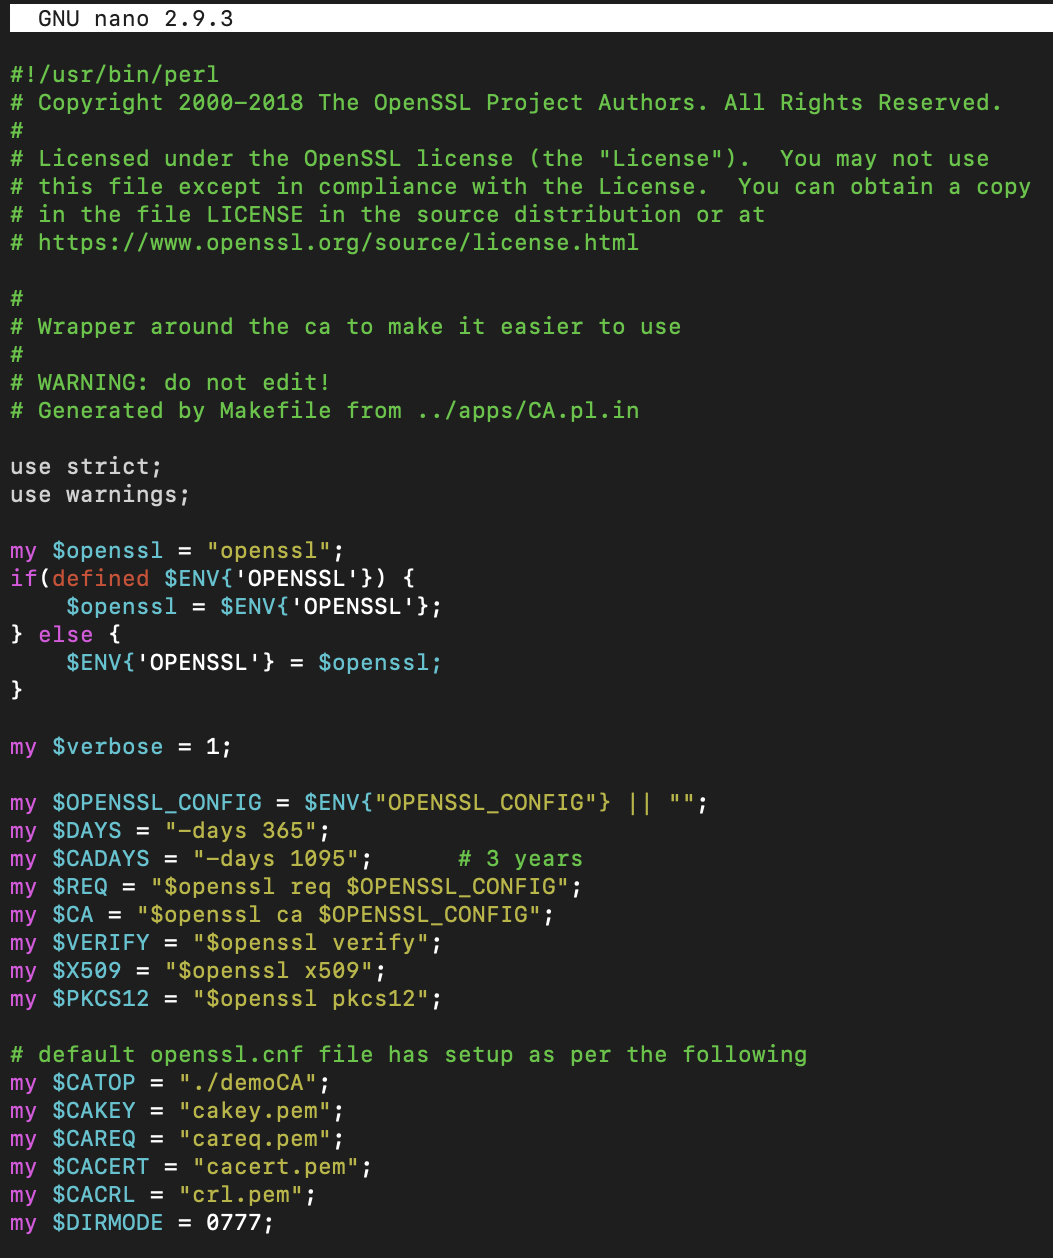
\includegraphics[width=0.5\textwidth]{pic1-hw6-7-1635747.png}
 \label{fig:capl}
\end{figure}

Now we have to make the same change also in the openssl configuration file, in \texttt{/usr/lib/ssl/openssl.cnf}

\begin{figure}[!ht]
 \centering
 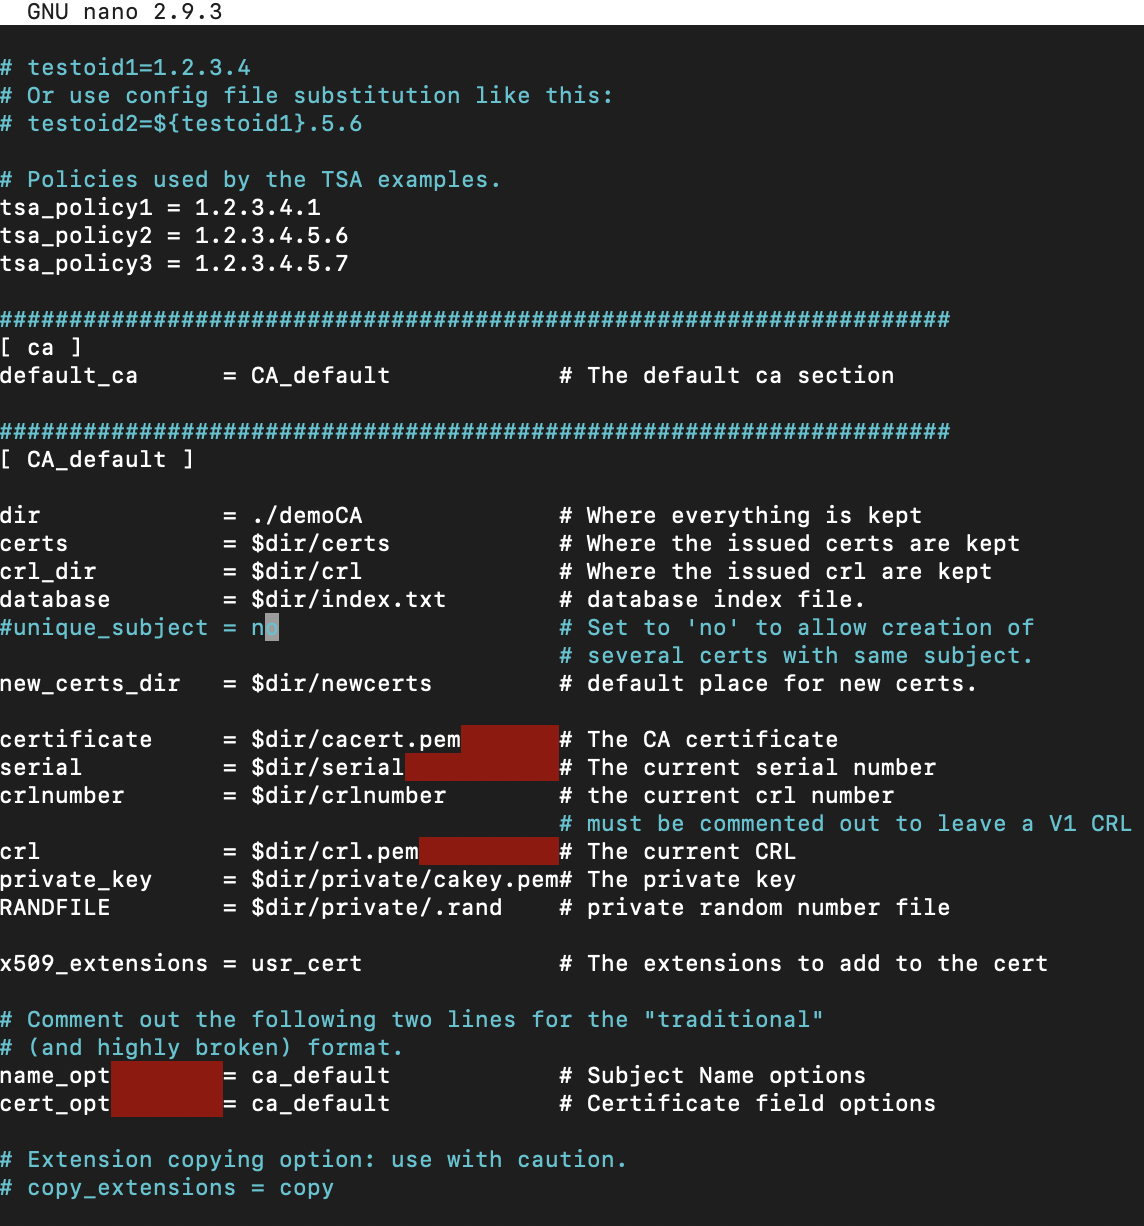
\includegraphics[width=0.5\textwidth]{pic2-hw6-7-1635747.png}
 \label{fig:conf}
\end{figure}

In these files, we find also the main pieces of information about the CA like the duration of the CA and the generated certificates.

\newpage
Now we are ready to create our CA with the following command:

\begin{quote}
 \texttt{/usr/lib/ssl/misc/CA.pl -newca}
\end{quote}

Following all the steps we have this results:

\begin{figure}[!ht]
 \centering
 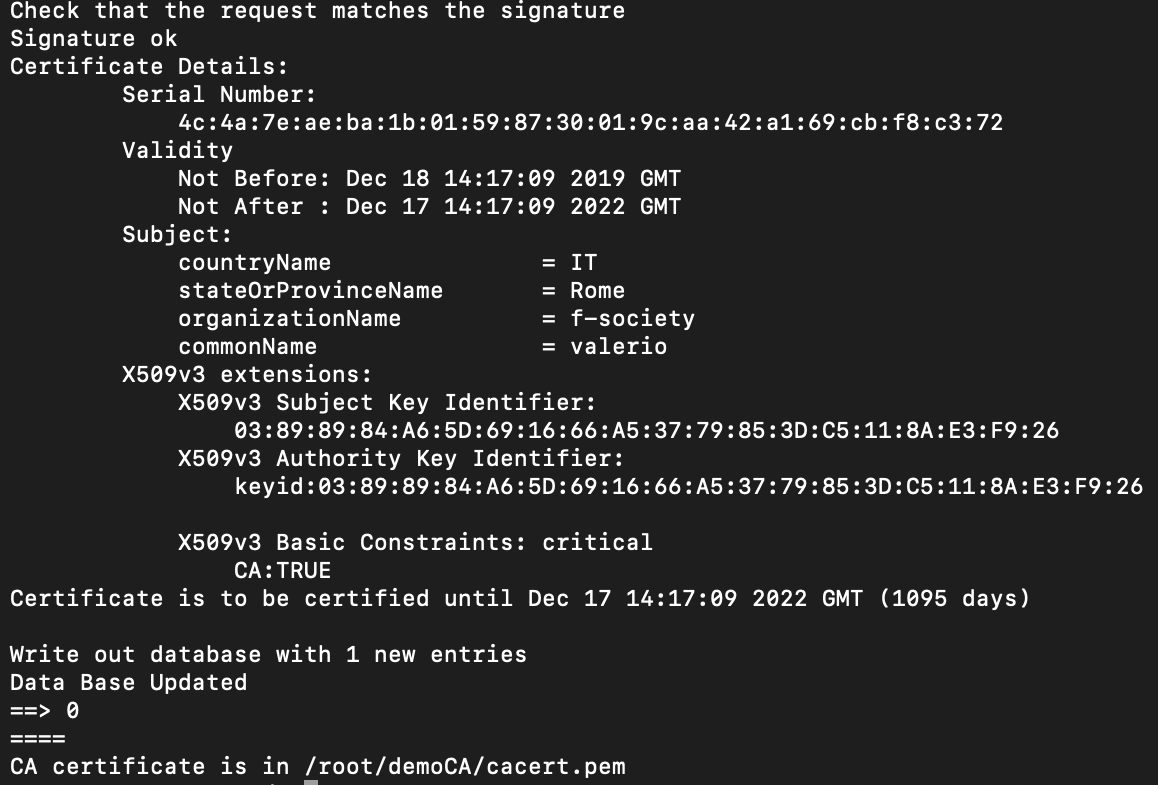
\includegraphics[width=0.8\textwidth]{pic3-hw6-7-1635747.png}
 \label{fig:results}
\end{figure}

This commands generate the CA certificate in the path \texttt{/root/demoCA/ cacert.pem}. Meanwhile the encrypted private key is saved in the path: \texttt{/root/demoCA/private/cakey.pem}. Ok now we have a certification authority that is able to validate and revoke certificates. But after to start the communication analyze a bit the folder {\em demoCA}:

\begin{figure}[!ht]
 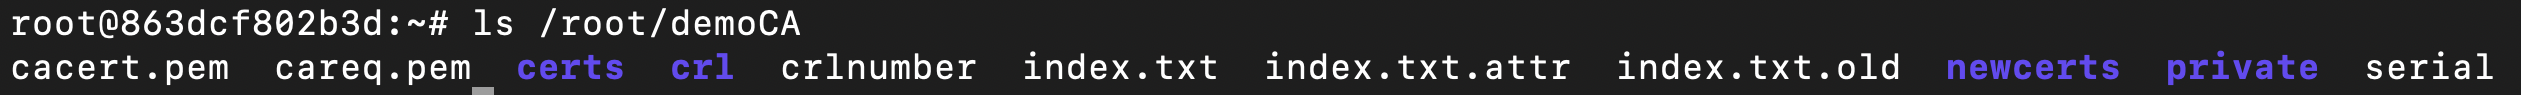
\includegraphics[width=1\textwidth]{pic4-hw6-7-1635747}
 \label{fig:demoCA}
\end{figure}

this is the structure and this is important to know it because all the certificates will be saved in this folder: {\em careq.pem} is the request for itself to subsign the certificate, {\em certs} directory has the trusted certificate, {\em crl} and {\em crlnumber} are the certification revocation list folder and number, {\em index.txt.att} is the database of certificates, in {\em newcerts} will be starting the new certificates that we validate from this CA, {\em private} folder has the key pair, and finally {\em serial} is the serial number of the CA.

\newpage
\subsection{Experimentation}
In the next steps, we simulate the request to sign a certificate and the request to validate a certificate.

\subsubsection{Certificate signing request (CSR)}

\begin{figure}[!ht]
 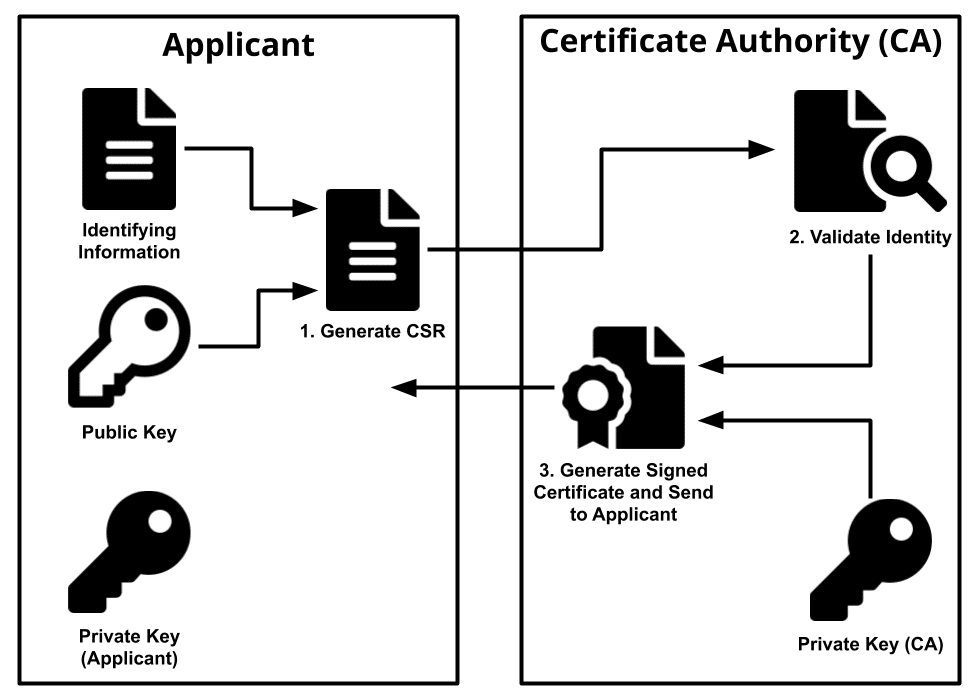
\includegraphics[width=.98\textwidth]{pic5-hw6-7-1635747}
 \label{fig:CA sign certificate}
\end{figure}

What we do in this section is represented in the figure above. We have our VM with a CA configured and on the other side have Alice's VM. The following are the main steps:
\begin{enumerate}
 \item CA wait for a request:\newline
 \texttt{\$ nc -l -p [CA port] > alice-req.pem}

 \item Alice generate a Certificate signing request (CSR) and send it to CA:\newline
 \texttt{\$ openssl req -new -keyout alice-keys.pem -out alice-req.pem}\newline
 \texttt{\$ pv alice-req.pem | nc [CA ip] [CA port] -q 5}

 \begin{figure}[!ht]
 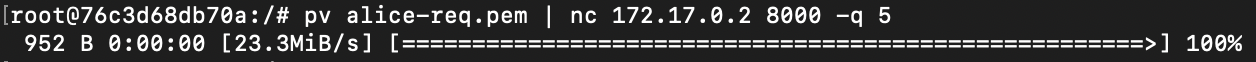
\includegraphics[width=1\textwidth]{pic6-hw6-7-1635747}
 \label{fig:pv result}
 \end{figure}

 \item CA check that the request matches the signature, sign the certificate and finally add it to the database:\newline
 \texttt{\$ openssl ca -in alice-req.pem}\newline
 now this generates a new certificate in the folder \texttt{/demoCA/newcerts} where the certificates are named automatically by the CA with a hexadecimal number. The last generated certificate is the one with the biggest number.

 \item Alice wait for the signed certificate:\newline
 \texttt{\$ nc -l -p [Alice port] > alice-cert.pem}

 \item CA send back the signed certificate:\newline
 \texttt{\$ pv alice-cert.pem | nc [Alice ip] [Alice port] -q 5}
\end{enumerate}

\subsubsection{Certificate revocation}
For any reason, a CA can decide to revoke a certificate before its expiry. In OpenSSL this procedure is very simple, in fact in the CA VM just run the commands:

\begin{enumerate}
 \item CA revokes the certificate:\newline
 \texttt{\$ openssl ca -revoke demoCA/newcerts/number\_of\_cert.pem}

 \item CA updates the certificates revocation list:\newline
 \texttt{\$ openssl ca -gencrl -out demoCA/crl/crl.pem}\newline
\end{enumerate}

\subsubsection{Certificate validation}
The last step we will face is the verification of the certificate. This procedure is very important for a secure communication. The simple way to do this is:

\begin{enumerate}
 \item CA wait for a request:\newline
 \texttt{\$ nc -l -p [CA port] > alice-req.pem}

 \item Alice send her own certificate to the CA:\newline
 \texttt{\$ pv alice-cert.pem | nc [CA ip] [CA port] -q 5}

 \item CA verifies the certificate trough its own certificate:\newline
 \texttt{\$ openssl verify -CAfile demoCA/cacert.pem}\newline
 \texttt{demoCA/newcerts/alice-cert.pem}
\end{enumerate}

If the verification successed then we have the output:

\texttt{demoCA/newcerts/alice-cert.pem: OK}.

\bigskip
But this verification is not complete because it verifies only the validation of the signature and the deadline of the certificate. The issue is that even if this last two are correct the certificate could be not valid because it could be revocated in the past. For this reason, we change this last command to verify also the revocation:

\begin{quote}
 \texttt{\$ openssl verify -CAfile demoCA/cacert.pem -CRLfile demoCA/crl/crl.pem -crl\_check demoCA/newcerts/alice-cert.pem}
\end{quote}

If this verification succeeds the certificate is valid and not revocated, instead if the certificate has been revocated the output will be like that:\newline

\begin{figure}[!ht]
 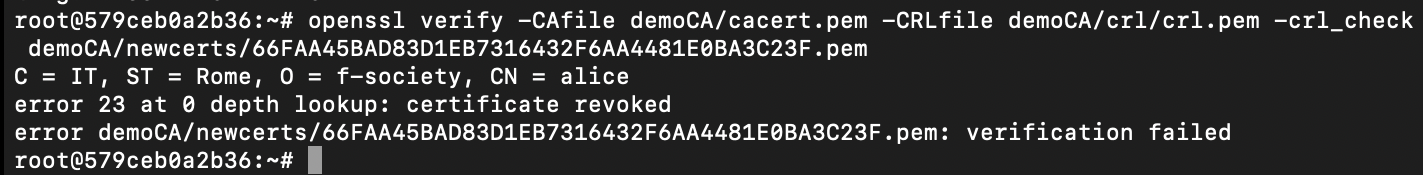
\includegraphics[width=1\textwidth]{pic7-hw6-7-1635747}
 \label{fig:crl result}
\end{figure}
We end here our adventure with public key cryptography with OpenSSL.


\vfill
\begin{thebibliography}{99}

\bibitem{doc}
{\em OpenSSL Documentation}. \newline
\verb|https://www.openssl.org/docs/manmaster/man3/|

\bibitem{doc2}
{\em Docker Documentation} \newline
\verb|https://docs.docker.com|

\bibitem{link2}
{\em Cryptography basics in OpenSSL}. \newline
\verb|https://opensource.com/article/19/6/cryptography-basics-openssl-part-2|

\bibitem{link3}
{\em Using Netcat for File Transfers} \newline
\verb|https://nakkaya.com/2009/04/15/using-netcat-for-file-transfers/|

\bibitem{video}
{\em Create and manage certificates and certification authorities} \newline
\verb|https://www.youtube.com/watch?v=uo_xz6sA4dY&t=11s|

\end{thebibliography}

\end{document}